%%%%%%%%%%%%%%%%%%%%%%%%%%%%%%%%%%%%%%%%%%%%%%%%%%%%%%%%
\fondo{celeste}
\section{Introducción}
\fondo{blanco}
%%%%%%%%%%%%%%%%%%%%%%%%%%%%%%%%%%%%%%%%%%%%%%%%%%%%%%%%

%%%%%%%%%%%%%%%%%%%%%%%%%%%%%%%%%%%%%%%%%%%%%%%%%%%%%%%%
\begin{frame}
    % \begin{columns}
    % \column{.6\textwidth}
  
    % \column{.4\textwidth}
        \begin{center}
        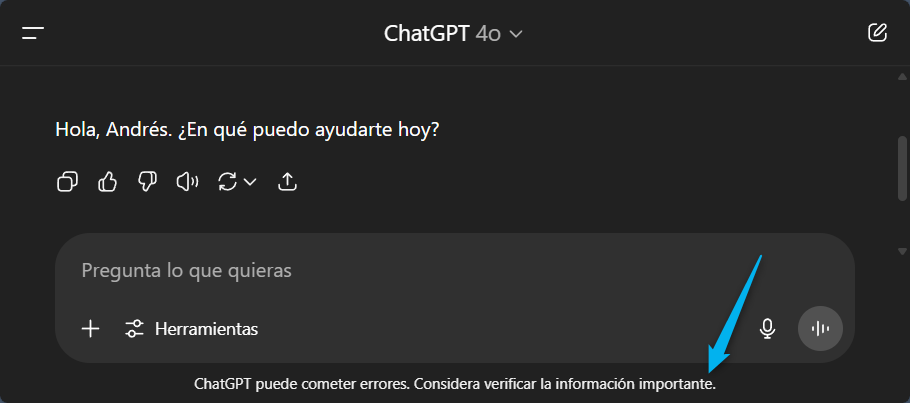
\includegraphics[width=0.8\linewidth]{Figuras/Fig01.png}
        \end{center}
    % \end{columns}
    \begin{block}{}\centering\large
        ChatGPT puede cometer errores: ¿prohibimos su uso en aula o lo aprovechamos para enseñar?
    \end{block}    
\end{frame}

\begin{frame}
    \begin{block}{Objetivo de la charla}
        \begin{itemize}[leftmargin=*]
            \item Reflexionar sobre el funcionamiento de ChatGPT y su tendencia a generar respuestas incorrectas.
            \item Presentar una experiencia concreta en el aula donde las alucinaciones se usaron como recurso didáctico.
            \item Explorar el diseño de GPTs personalizados que inducen errores con fines pedagógicos.
        \end{itemize}
    \end{block}

    \vspace{0.3cm}
    \pause
    \begin{block}{}\centering
        Caso de uso: Cálculo Diferencial
    \end{block}
\end{frame}



